\chapter{Stability}
\label{Stability}

\setlength{\epigraphwidth}{.9\textwidth}

\epigraph{It may be urged that change in language is due ultimately to the deviations of individuals from the rigid system. But it appears that even here individual variations are ineffective; whole groups of speakers must, for some reason unknown to us, coincide in a deviation, if it is to result in a linguistic change.\\ -- Leonard Bloomfield \citeyearpar[445]{bloomfield1927}}


%All this, de Saussure's la parole, lies beyond the power of our science. We cannot predict whether a certain person will speak at a given moment, or what he will say, or in what words and other linguistic forms he will say it. Our science can deal only with those features of language de Saussure's la langue, which are common to all the speakers of a community,?the phonemes, grammatical categories, lexicon, and so on. 

Distinguishing between the formal and functional Jespersen cycles simplifies the task of explanation. It allows us to disentangle two phenomena that overwhelmingly co-occur, and address them separately. For example, in the previous chapter we showed that the functional cycle in English can be explained in terms of the difficulty speakers have in keeping track of private versus common knowledge.  Crucially, this explanation of the transition from pre-verbal \emph{\textcolor{red}{ne}} to embracing \emph{\textcolor{blue}{ne...not}} rests on the way our pragmatic competence shapes the use and interpretation of linguistic signals over time. 

However, it is important to distinguish between the logical relationship between the two cycles and the explanation of a particular historical change. That is, the functional cycle can occur independently of the formal cycle, so we need an explanation for cases where it does occur independently. But, in the case of English, and many other languages, the functional cycle coincides with the first transition of the formal cycle. There is no guarantee that the model we described to address the functional cycle is the only or even the best explanation of the observed transitions of the formal cycle. That is, in any given case, pragmatic pressures might not explain the first transition of the formal cycle.

Here we consider other potential explanations for both of the transitions of the formal cycle.  In particular, we examine the possible role of acquisition. The facts to be explained are the transition from pre-verbal \emph{\textcolor{red}{ne}} to embracing \emph{\textcolor{blue}{ne...not}} and the transition from embracing \emph{\textcolor{blue}{ne...not}} to post-verbal \emph{\textcolor{green}{not}}. Our goal is to understand whether the process of acquisition offers any insights into why the formal cycle takes place. More broadly, we want to test whether grammatical competence and the process by which it is formed are sufficient to explain the observed changes.

First, we present a model of syntactic acquisition that has several desirable theoretical properties. Second, we determine the dynamics of the model in a population over time. In particular, we show the conditions under which the acquisition dynamics lead to change or stable variation. Third, we outline the syntactic structures at various stages of the formal cycle. These structures allow us to explicitly state the conditions for the acquisition dynamics to lead to either of the transitions of the formal cycle. Finally, we fit the model of the acquisition dynamics to data from the formal cycle in Middle English and discuss the implications of the fitted parameters.  

Acquisition can be taken as a cause of the formal cycle if only if the following qualitative and quantitative criteria are met. First, given the acquisition dynamics and grammatical structures underlying the formal cycle, we should predict the qualitative occurrence of both transitions. Second, if the acquisition dynamics predict the transitions, then the quantitative parameters of the dynamics fit to corpus data should be consistent with our theoretical assumptions. That is, the parameters of the model have some falsifiable empirical content that can be tested using corpus data. If neither of these criteria are met, then acquisition cannot explain the transitions of the formal cycle.

In fact, we show that neither of the transitions of the formal cycle observed in the history of English can be explained by acquisition. First, for the grammatical structures posited to underly the formal cycle the acquisition dynamics predict stability rather than change.  So, the first criterion cannot be met. Second, this also means that the second criterion cannot be met either; given that both transitions do occur, the parameters of the fitted model necessarily differ. In fact, it would seem that the only way acquisition could lead to either of the transitions would be, in Bloomfield's terms, a mass coincidence of deviation from the current system.

The main contributions of this chapter are twofold. First, we offer a general analysis of the acquisition dynamics, which clearly delineates the conditions for stability and change under certain kinds of parametric variation. Second, we make explicit the conditions for acquisition to play a role in either of the transitions of the formal cycle. In particular, one must show not only that acquisition predicts both transitions qualitatively, but that it also matches the quantitative trajectory of the change. It is important to note that these hold for any set of syntactic structures posited to underly the formal cycle. Demonstrating the role of acquisition requires demonstrating how the acquisition dynamics leads from one state to another.


\section{A model of acquisition}

In the most general sense, the process of language acquisition is some mapping from the initial state of the learner and the linguistic evidence provided to the learner to some terminal state, which is taken to be the grammatical competence of the speaker. We begin by introducing a model that can be used to describe this process. We then note some of the properties that make it an appealing model of acquisition.

The \emph{variational learning} model of acquisition \citep{yang2000internal,yang2002} consists of three basic components. First, there is a finite set of grammars that vary in a parametric fashion, in the sense of the  \emph{Principles and Parameters} framework \citep{chomsky1981,chomsky1995,chomsky-lasnik1993}. Second, a learner keeps track of a probability distribution over grammars, which we can think of as the weights of evidence the learner has for the various grammars. Third, a learner updates her distribution over grammars according to a learning scheme as she receives input from the linguistic environment.

To see this in detail, suppose that a learner is presented with sentences from the linguistic environment. The learner selects a grammar $G_i \in G = \{G_1,...,G_n \}$ with probability $p_i$ to analyze a sentence. There are two possible outcomes: either the grammar can analyze the sentence or it cannot. That is, the sentence is grammatical with respect to the selected grammar or it is not. The learner updates her distribution over grammars in the following manner, where $0 < \gamma \ll 1$ is a small learning parameter.


\begin{equation}
 \mbox{If $G_i \rightarrow s$ then }
\left\{
	\begin{array}{ll}
		p_i'  = (1 - \gamma)p_i + \gamma \\
		p_j'  = (1-\gamma)p_j & \mbox{for} j \neq i
	\end{array}
\right.
\end{equation}

\begin{equation}
 \mbox{If $G_i \nrightarrow s$ then }
\left\{
	\begin{array}{ll}
		p_i'  = (1-\gamma ) p_i \\
		p_j'  = (1-\gamma)p_j + \frac{\gamma}{n - 1} & \mbox{for} j \neq i
	\end{array}
\right.
\end{equation}
This is a \emph{linear reward-punishment} scheme \citep{bush-mosteller1955}:\footnote{This learning scheme is similar to the linear reward-inaction scheme that yields the replicator dynamics \citep{borgers-sarin1997}. It differs in that failures are not ignored, but rather punished. One compelling reason for treating learning differently across the domains of meaning and structure is the hypothesis space of each: the grammatical hypothesis space is heavily constrained, whereas the semantic hypothesis space, even under the Fodorian \citeyearpar{fodor1975} conception, is constrained but arguably unbounded. That is, even a finite set of innate concepts can be combined in the appropriate manner without end. Given this quantitative, if not qualitative difference between the domains, it is not clear how a learner would decide what aspects of a given hypothesized meaning to punish (cf. \citealt{quine1960}). But, see \cite{smith-yu2008,medina-etal2011,smith-etal2011, trueswell-etal2013} for experimental evidence, and \cite{yu-smith2007,frank-etal2009,stevens-etal2013} for computational approaches to the problem of learning meaning.} grammars that are compatible with a sentence drawn from the linguistic environment are rewarded, whereas grammars that are not compatible with the sentence are punished. Both of these actions are reflected in the first line of the two possible outcomes. If the grammar can analyze the sentence, then its probability is bumped up by some small amount determined by the learning parameter. If the grammar cannot analyze the sentence, then its probability is knocked down by some small amount determined by the learning parameter. The second conditions allow for the weights over grammars to be redistributed while guaranteeing that all probabilities always sum to one.

Now, the probability that a learner attributes to a grammar changes according to how successful that grammar is in dealing with the linguistic environment. In fact, the long term distribution over grammars can be determined from the probability that a grammar will not be able to analyze a sentence and will thus be penalized. For two grammars, $G_1$ and $G_2$, let the \emph{penalty probabilities} be $c_1$ and $c_2$, respectively. It can be shown that the expected value of the probabilities of the two grammars converge to the following limit values \citep[111]{narendra2012}.
\begin{equation}
\begin{split}
\lim_{t \rightarrow \infty} E[p_1(t)] &= \frac{c_2}{c_1 + c_2 }\\
\lim_{t \rightarrow \infty} E[p_2(t)] &= \frac{c_1}{c_1 + c_2 }
\end{split}
\end{equation}
We should note that this result is about the expected behavior of an individual, rather than the actual behavior of that individual. So, while the expected value of the probabilities converges to these values, the actual probability in the mind of a given learner does not. As we will see below, the actual values in the mind of an individual are close to, but not necessarily equal to these values. This distinction has important implications for the dynamics of acquisition, which we return to in the next section. In particular, it requires us to make certain assumptions about the size of the population.

%Second, the expected value of the probability of a grammar in the limit is directly proportional to the penalty probability of that grammar. Importantly, this means that learners get the appropriate ordering of weights to evidence, which is a property we would arguably expect of any learning model.

%�\footnote{This property holds for an arbitrary number of grammars \citep[117]{narendra2012}.}

So, we know the expected behavior of a learner given the penalty probabilities of the grammars in question. We can determine the penalty probabilities in the following manner. First, suppose that the linguistic environment is composed of the output of two partially incompatible grammars. Let $\alpha_1$ be the proportion of sentences generated at random by the first grammar $G_1$ that the second grammar $G_2$ cannot analyze; likewise let $\alpha_2$ be the proportion of sentences generated at random by the second grammar $G_2$ that the first grammar $G_1$ cannot analyze. Note that while the assumptions underlying them are theoretical both $\alpha_1$ and $\alpha_2$ empirical estimates of both can be calculated from a corpus (e.g. \citealt[94-95]{ingason-etal2013}).  We can represent the relationship between the two grammars visually as in Figure \ref{grammars-evidence} where the overlap of the two grammars indicate the sentences that are jointly analyzable by both grammars.  Second, let the linguistic environment be composed of some distribution over the two grammars, call it $L = p_1G_1 + p_2G_2$.  From this we can calculate the penalty probabilities as $c_1 = p_2\alpha_2$ and $c_2 = p_1\alpha_1$. The likelihood that the first grammar will not be able to analyze a sentence depends on the prevalence of the second grammar in the environment and the likelihood a sentence generated by that second grammar will be incompatible with the first grammar. The same reasoning holds for the second grammar. 

%That is, the likelihood that each of the grammars will not be able to analyze a sentence depends on the independent evidence for the other grammar and its prevalence in the environment.


\begin{figure}
\begin{center}
        \begin{tikzpicture}
	  \node (A) [draw,circle,minimum size=4cm]  at (0,0) {$\alpha_1$};
	  \node (G1) [above of=A] {$G_1$};
	  \node [draw,circle,minimum size=4cm] (B) at (0:3cm) {$\alpha_2$};
	  \node (G2) [above of=B] {$G_2$};
	\end{tikzpicture}         
    \end{center}
\caption{Two partially incompatible grammars}
\label{grammars-evidence}
\end{figure}

We can get a sense for the learning process by simulating individual trajectories. This can be seen in Figure \ref{lrp-learning} where the horizontal axis represents time as additional sentences drawn from the environment and presented to the learner. The vertical axis represents the weight of $G_2$ in the learner's mind. We can compare the expected motion averaged across several hundred individual trajectories in bold to several individual trajectories. Where the expected motion smoothly approaches the value predicted by the model, shown by the dotted line, individual trajectories continue to move around the value. Again, we return to this important distinction in the next section when we turn to the dynamics of the model.

\begin{figure}
\begin{center}
	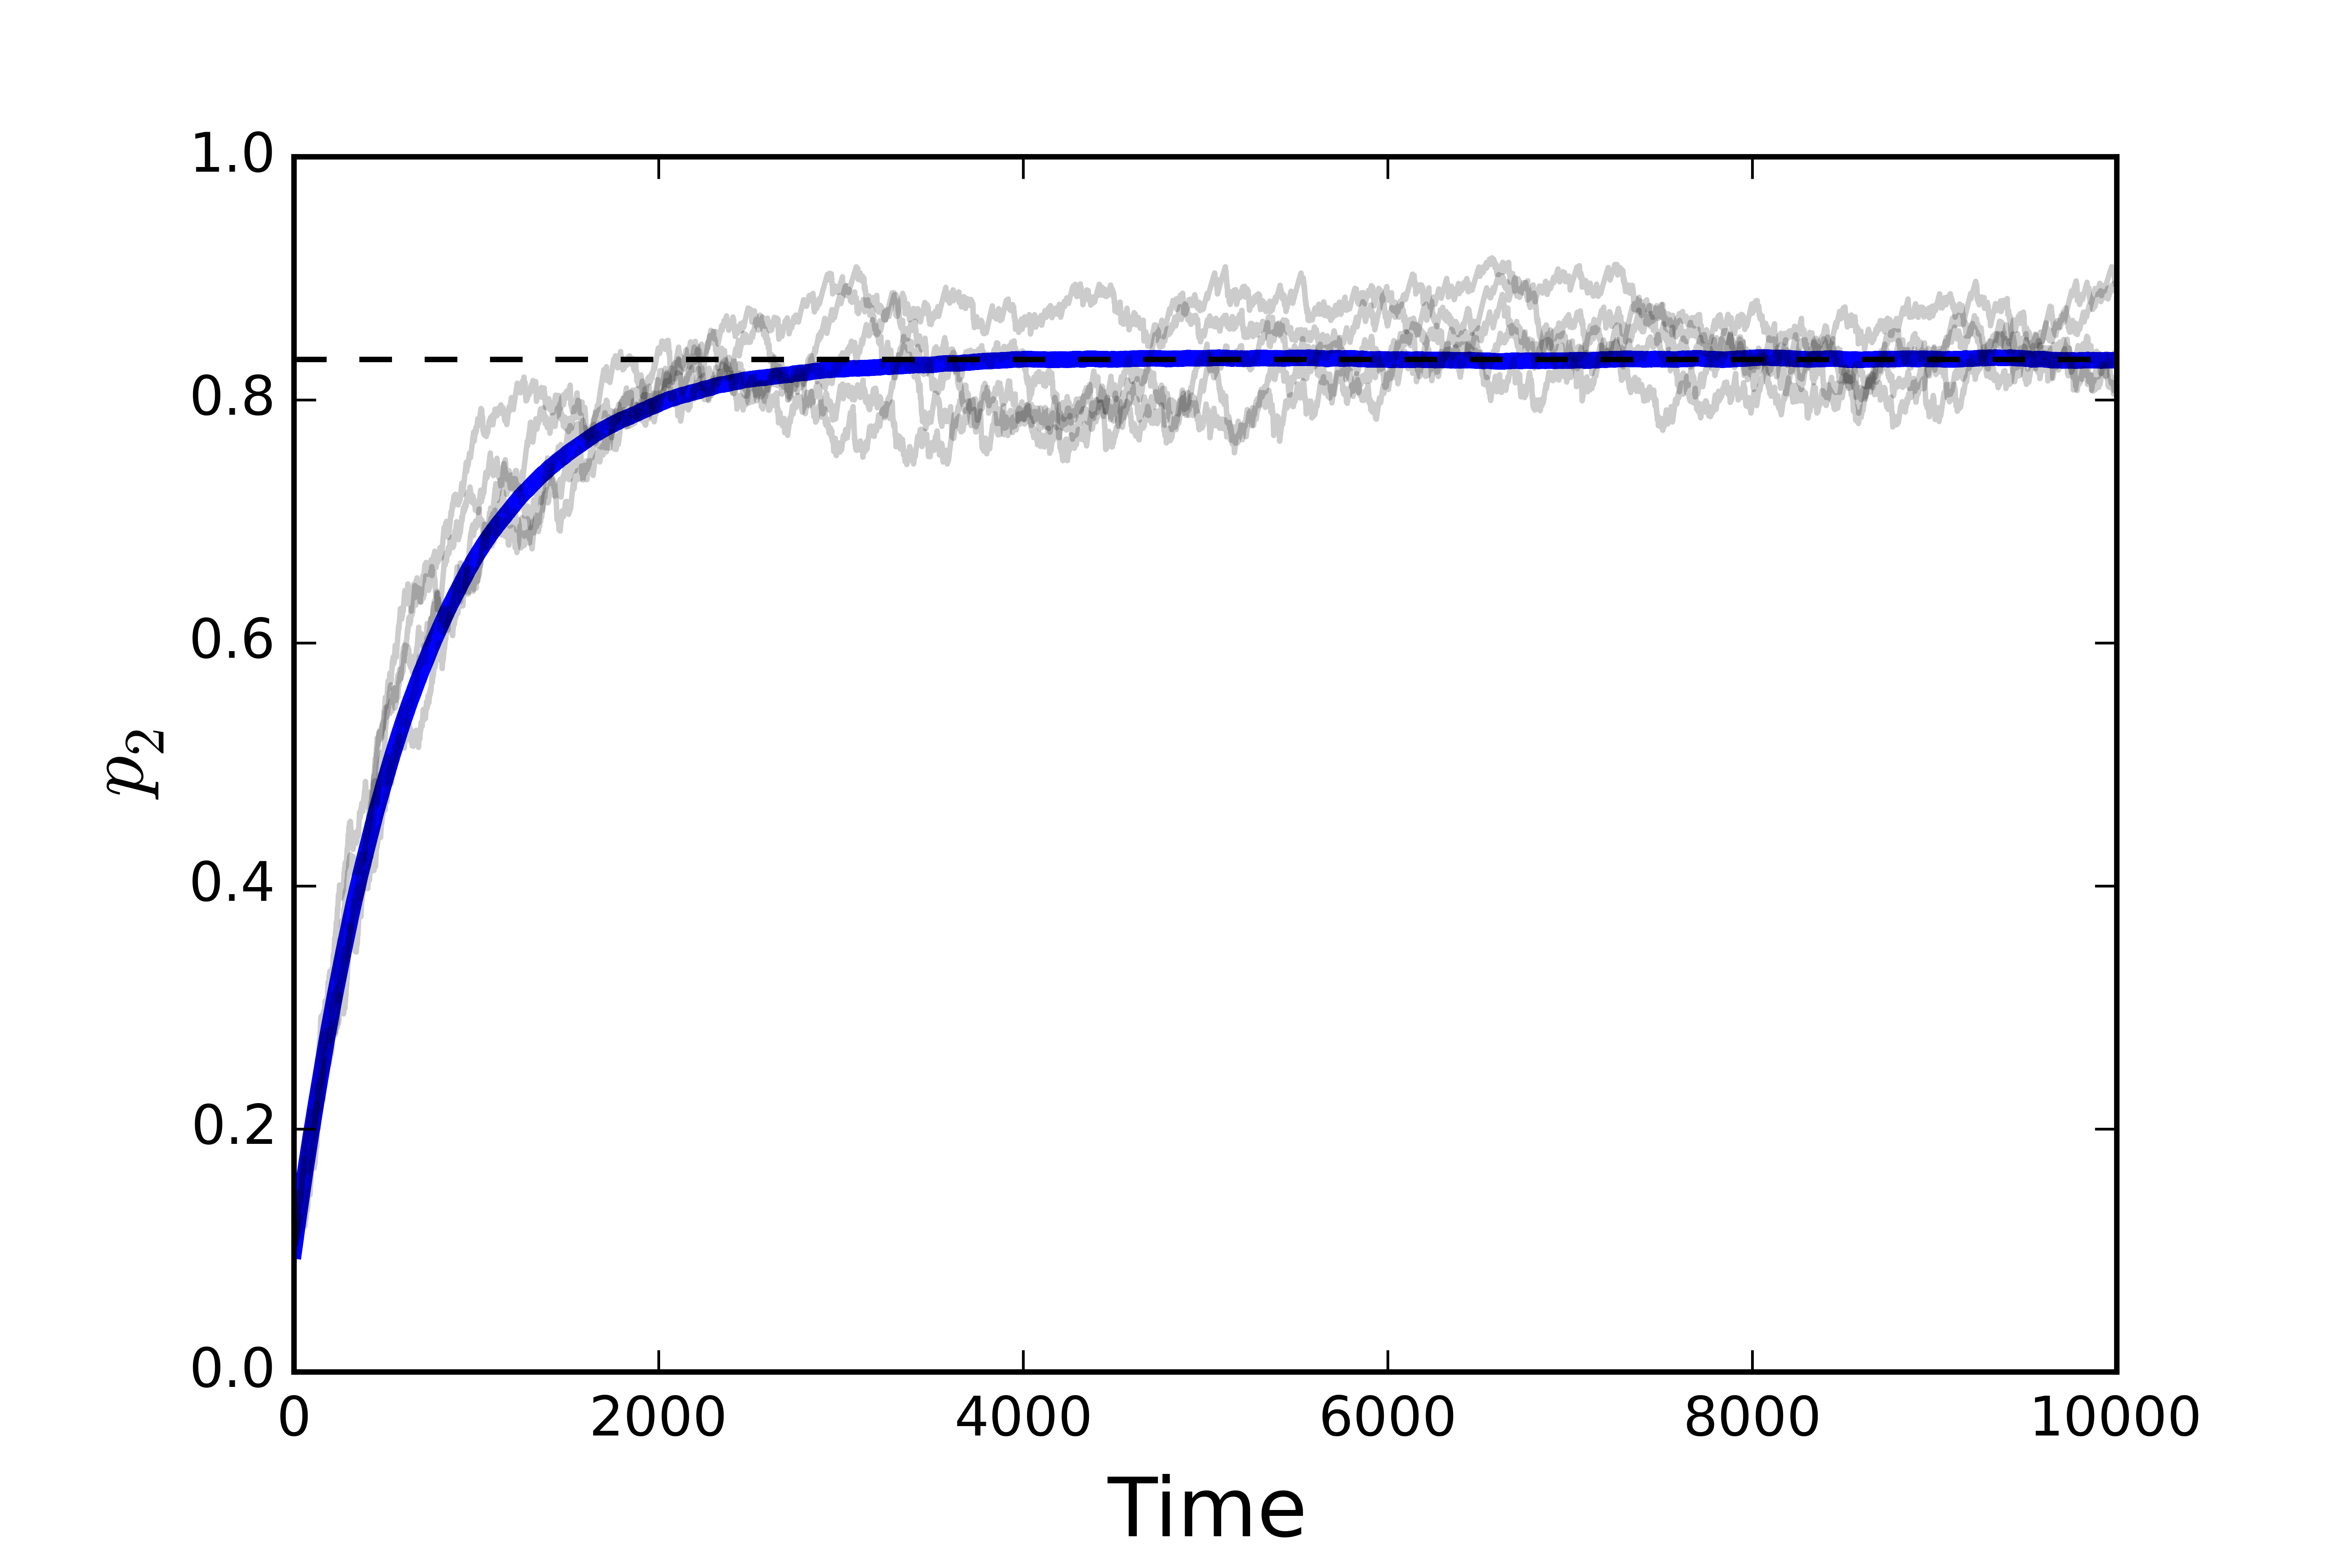
\includegraphics[width=.75\textwidth]{lrp-learning.png}\\
\end{center}
	\caption{Probability of $G_2$ over time for various individual trajectories and expected motion of trajectories, where $L=\frac{1}{2}G_1 + \frac{1}{2}G_2$,  $\alpha_1 = .1, \alpha_2 = .5, \gamma=.1$}
	\label{lrp-learning}
\end{figure}

However, before doing so, there are several important properties that are evident from the simulations presented in Figure \ref{lrp-learning}.  First, this learning model allows for the gradual adjustment of learners to the linguistic environment rather than abrupt changes (cf. \citealt{gibson-wexler1994,hyams-wexler1993}). Second, it allows learners to converge to distributions over grammars, rather than a single grammar \citep{kroch1989}. Third, the expected value of the probability of a grammar is directly proportional to its penalty probability  \citep[117]{narendra2012}, which means that learning is reasonably robust. These properties, along with the overall simplicity of the model make it an appealing starting point for investigating how acquisition might lead to change over time.


\section{The dynamics of acquisition}

We showed the properties of the variational learning model at the level of the individual; we now turn to the dynamics of learning in a population over time. First, we show how the expected change from one point in time to the next gives rise to a particular dynamics under particular assumption. Second, we show that the stable rest points of the dynamics are single grammars, with an important exception. We also show how these dynamics are closely related to the logistic model often taken as a proxy for changes in competing grammars.

Under the variational model, for the case of two grammars, we denote the expected value of the weight accorded to the grammar $G_2$ by a learner to be the following. That is, the average behavior of a learner converges to a probability determined by penalty probabilities and the prevalence of the two grammars in the linguistic environment.

\begin{equation}
p_2' = \frac{p_2 \alpha_2}{p_1 \alpha_1 + p_2 \alpha_2}
\end{equation}
Now, suppose that this distribution in turn serves as the linguistic environment for the next generation of learners. We can determine the expected change in the average weight of $p_2$ from one generation of learners to the next as the following.

\begin{equation}
\dot{p}_2 = p_2' - p_2 = \frac{p_2 \alpha_2}{p_1 \alpha_1 + p_2 \alpha_2} - p_2 = p_2(1-p_2)\frac{\alpha_2 - \alpha_1}{p_1 \alpha_1 + p_2 \alpha_2}
\end{equation}
This \emph{mean dynamics} follows the expected motion of the distribution over grammars in the population. Note that we are talking about the change in the expected behavior in the population. This means that we are modeling a fact about the population as a whole, which ultimately derives from individual learning. However, justifying the mean dynamics requires two important assumptions about the population.

The first assumption that must be made is about the size of the population. As we noted in the previous section, learners converge to the limit values only in expectation. In fact, an individual learner is almost always either slightly above or slightly below this expected value, as can be seen in Figure \ref{lrp-learning}. But, the distribution over these values in a population of learners at a given point in time is roughly normally-distributed around the limit value, as can be seen in Figure \ref{lrp-dist}. In this case, the expected value in the population is close to the limit value. As the population grows, the expected value in the population gets closer and closer to the limit value. In the limit of an infinite population, the linguistic environment for the next generation of learners is the limit value.\footnote{This is often a necessary assumption for studying the mean dynamics of what is undoubtedly a stochastic process. See Chapter 10 of \cite{sandholm2010} for a detailed derivation of the mean dynamics as the limit of a stochastic process in infinite population.    In the next chapter we relax the assumption of an infinite population, allowing for stochasticity in the change in the population over time.}
\begin{figure}
\begin{center}
	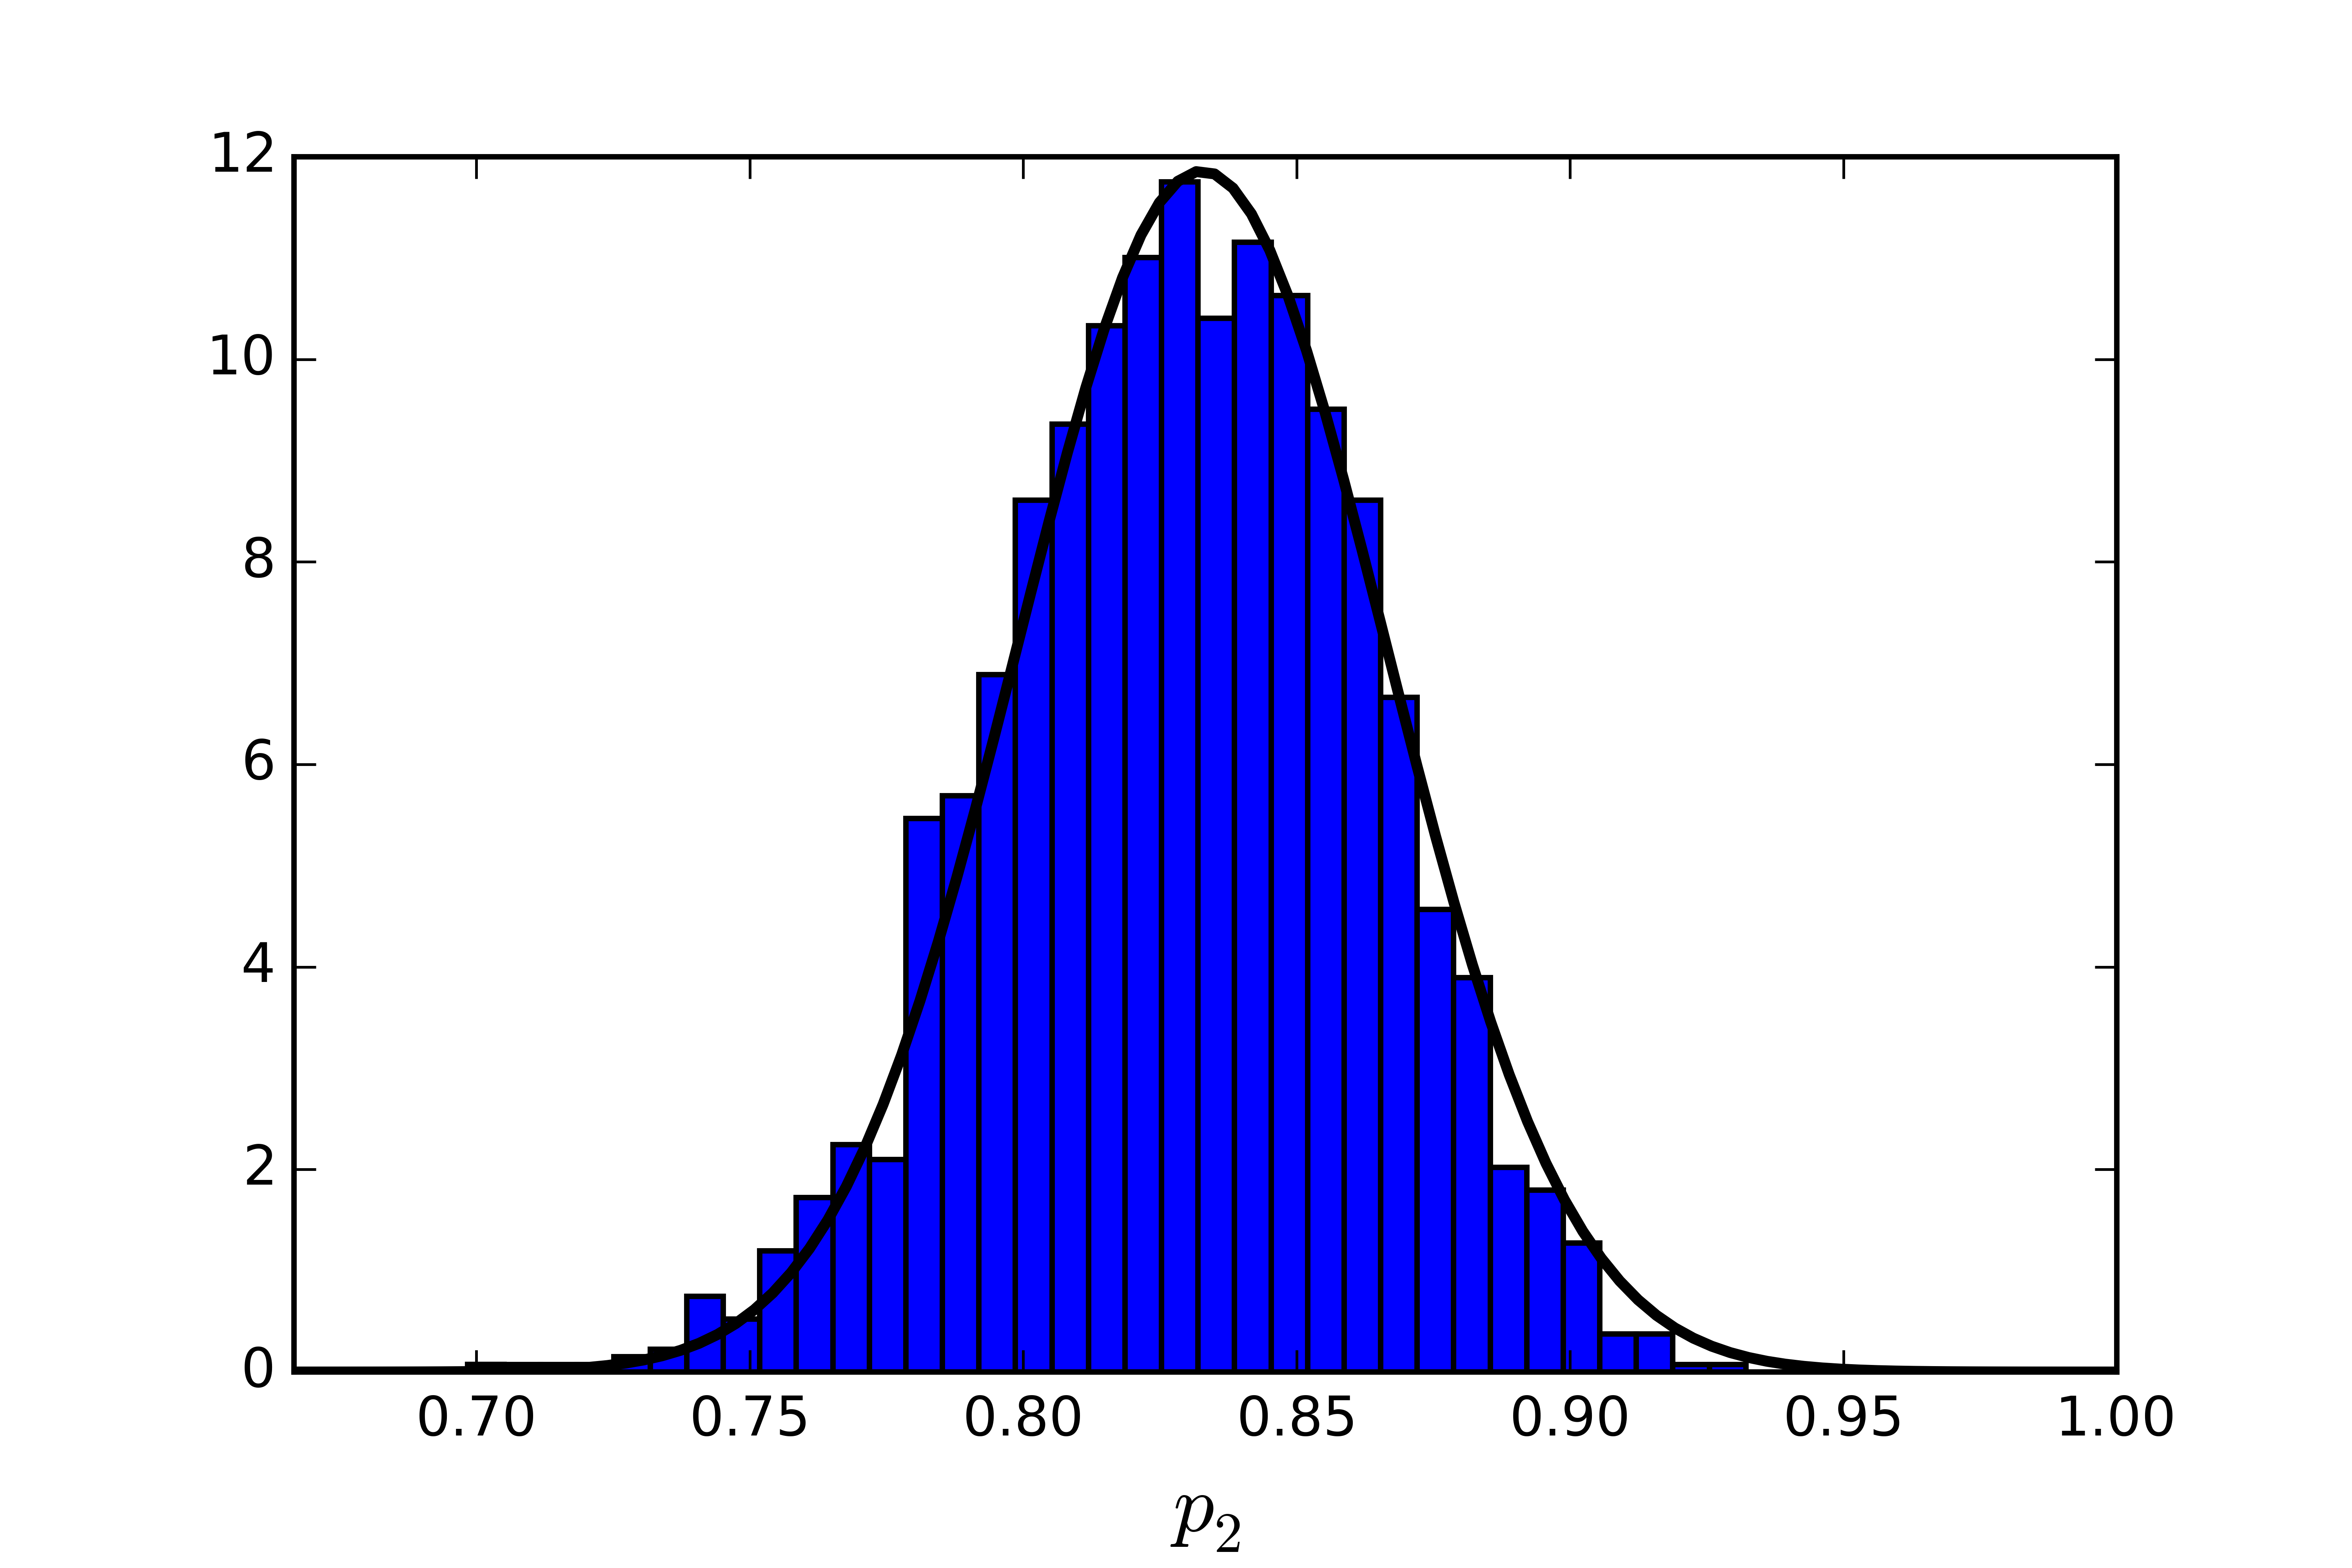
\includegraphics[width=.75\textwidth]{lrp-dist.png}\\
\end{center}
	\caption{Distribution over $p_2$ for population of learners and fitted normal distribution}
	\label{lrp-dist}
\end{figure}

The second assumption that must be made is about the structure of the population. Namely, the continuous-time form of the dynamics requires that we assume that there are continuously overlapping generations of learners that contribute to the linguistic environment.\footnote{A discrete-time dynamics might be more appropriate in allowing for a lag between when learners converge on a grammar and contribute to the linguistic environment, but this  distinction does not affect the subsequent results.} Together these assumptions guarantee that the dynamics track the expected weights over the grammars in the minds of learners over time. Thus, the solutions to this \emph{mean dynamics} is a model of the expected behavior in the population.

For the case of two grammars, we can simplify the dynamics in the following manner. Let $s = \frac{\alpha_2 - \alpha_1}{\alpha_2}$ and $p_2 = p$, then we have the following. In population genetics $s$ is referred to as the \emph{selection coefficient} of $\alpha_1$. For cases where $s > 0$,  $\alpha_2 $ has a selective advantage and $\alpha_1$ is selected against. For $s=0$, $\alpha_1$ and $\alpha_2$ are selectively \emph{neutral}.

\begin{equation}
\dot{p} = p(1-p)\frac{s}{1- s(1-p)}
\end{equation}
We can read the rest points off the resulting acquisition dynamics. There are two important cases that we will consider. First, if there is only a single grammar, then the weight over grammars is stable. That is, if $p=0$ or $p=1$, then the dynamics are, so to speak, at rest.  This makes intuitive sense, a grammar cannot be considered if there is no evidence for it. Second, if there is a perfectly balanced amount of independent evidence for both grammars $s = 0$, then any distribution over grammars is a rest point. This also makes intuitive sense, if the balance of evidence is equally in favor of both grammars, then things should not change. We determine the stability of these sets of rest points in turn.

For the first set of rest points, we can evaluate the stability of a single grammar as a function of the selection coefficient, which captures the ratio of independent evidence in favor of one or the other grammar. To do so we evaluate the derivative of the dynamics at the two rest points constituted by a single grammar. If the derivative evaluated at the rest point is negative, then the rest point is \emph{asymptotically stable}. That is, the dynamics will carry the population to the rest point. If the derivative evaluated at the rest point is positive, then the rest point is \emph{unstable}. That is, the dynamics will carry the population away from the rest point. We can express these conditions as a function of the selection coefficient, $s$. 

\begin{equation}
\frac{\partial \dot{p}}{\partial p} \big|_{p=0} = \frac{s}{1-s}
\end{equation}

\begin{equation}
\frac{\partial \dot{p}}{\partial p} \big|_{p=1} = -s
\end{equation}
Note that for $s \neq 0$, only one of these rest points can be asymptotically stable. The rest point $p=0$ is asymptotically stable if and only if $s < 0$. That is, the population will eventually use grammar $G_1$ exclusively if only if there is more evidence for it than there is $G_2$. The rest point $p=1$ is stable if and only if $s > 0$. That is, the population will eventually use grammar $G_2$ exclusively if and only if there is more evidence in favor of it. 

In fact, these conditions for the stability of both rest points are rather general. If we assume that the selection coefficient is not zero, then there are no other rest points. So, these conditions amount to conditions for \emph{global asymptotic stability}. Importantly, this means that no matter the initial distribution over grammars, if $s > 0$ then grammar $G_2$ will take over in the population. Thus, the acquisition dynamics are a kind of frequency-independent selection. We can get a sense for this fact by visualizing trajectories from the same low starting state of $p$ for various values of $s$ as in Figure \ref{lrp-gain}. No matter how small the initial proportion or slim the margin of evidence, it is guaranteed to eventually go to completion. 

%Under these dynamics, acquisition is a particularly robust process over time.

%\footnote{\citet[239]{yang2000internal} refers to this as the \emph{fundamental theorem of language change}.}

\begin{figure}
\begin{center}
 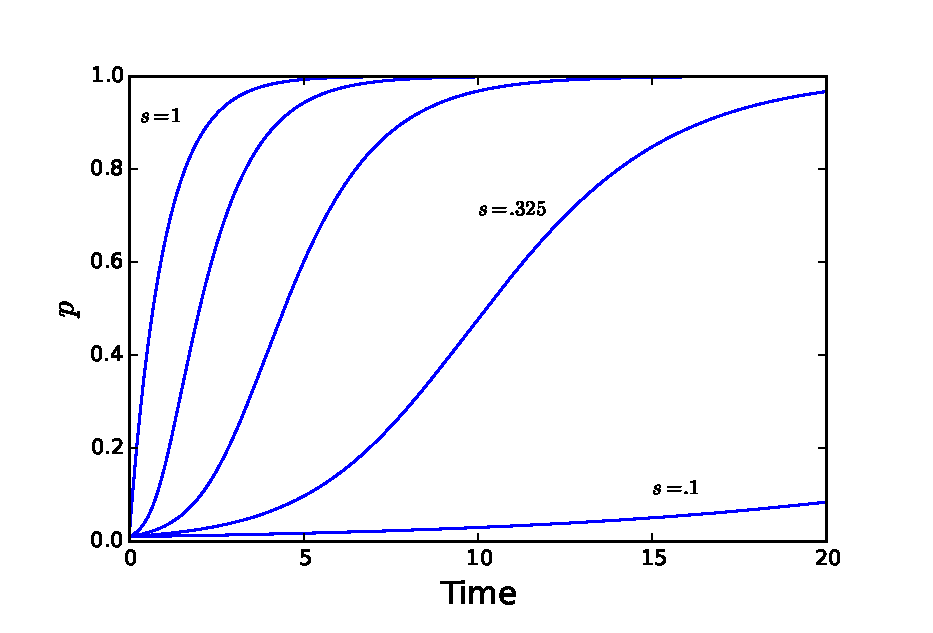
\includegraphics[width=.75\textwidth]{lrp-gain.eps}\\
\end{center}
	\caption{Proportion of $G_2$ over time for various ratios of evidence $s > 0$}
	\label{lrp-gain}
\end{figure}


Interestingly, the acquisition dynamics in these cases are closely related to the logistic models originally posited by \cite{altmann-etal1983} and \cite{kroch1989} to underly competing grammars. While there was no specific learning mechanism underlying the logistic model, it has both connections with the notion of biological competition as well as a straightforward application in terms of logistic regression (cf. \citealt[4]{kroch1989}). However, it is obvious that the variational model provides some justification for this conception when we compare the dynamics of logistic growth with the acquisition dynamics, where $s$ is taken as the growth rate in the logistic model.

\begin{equation}
	\dot{p} = p(1-p)s
\end{equation}
In fact, the only difference is that the acquisition dynamics exhibits a varying growth rate as a function of the distribution over grammars in the population. We show the solution for the acquisition dynamics and the logistic model from the same starting point with the same growth rate in Figure \ref{lrp-log}. The solution to the acquisition dynamics predicts a faster initial rate of growth, but slows down to the same rate as the logistic as $p \approx 1$.

\begin{figure}
\begin{center}
 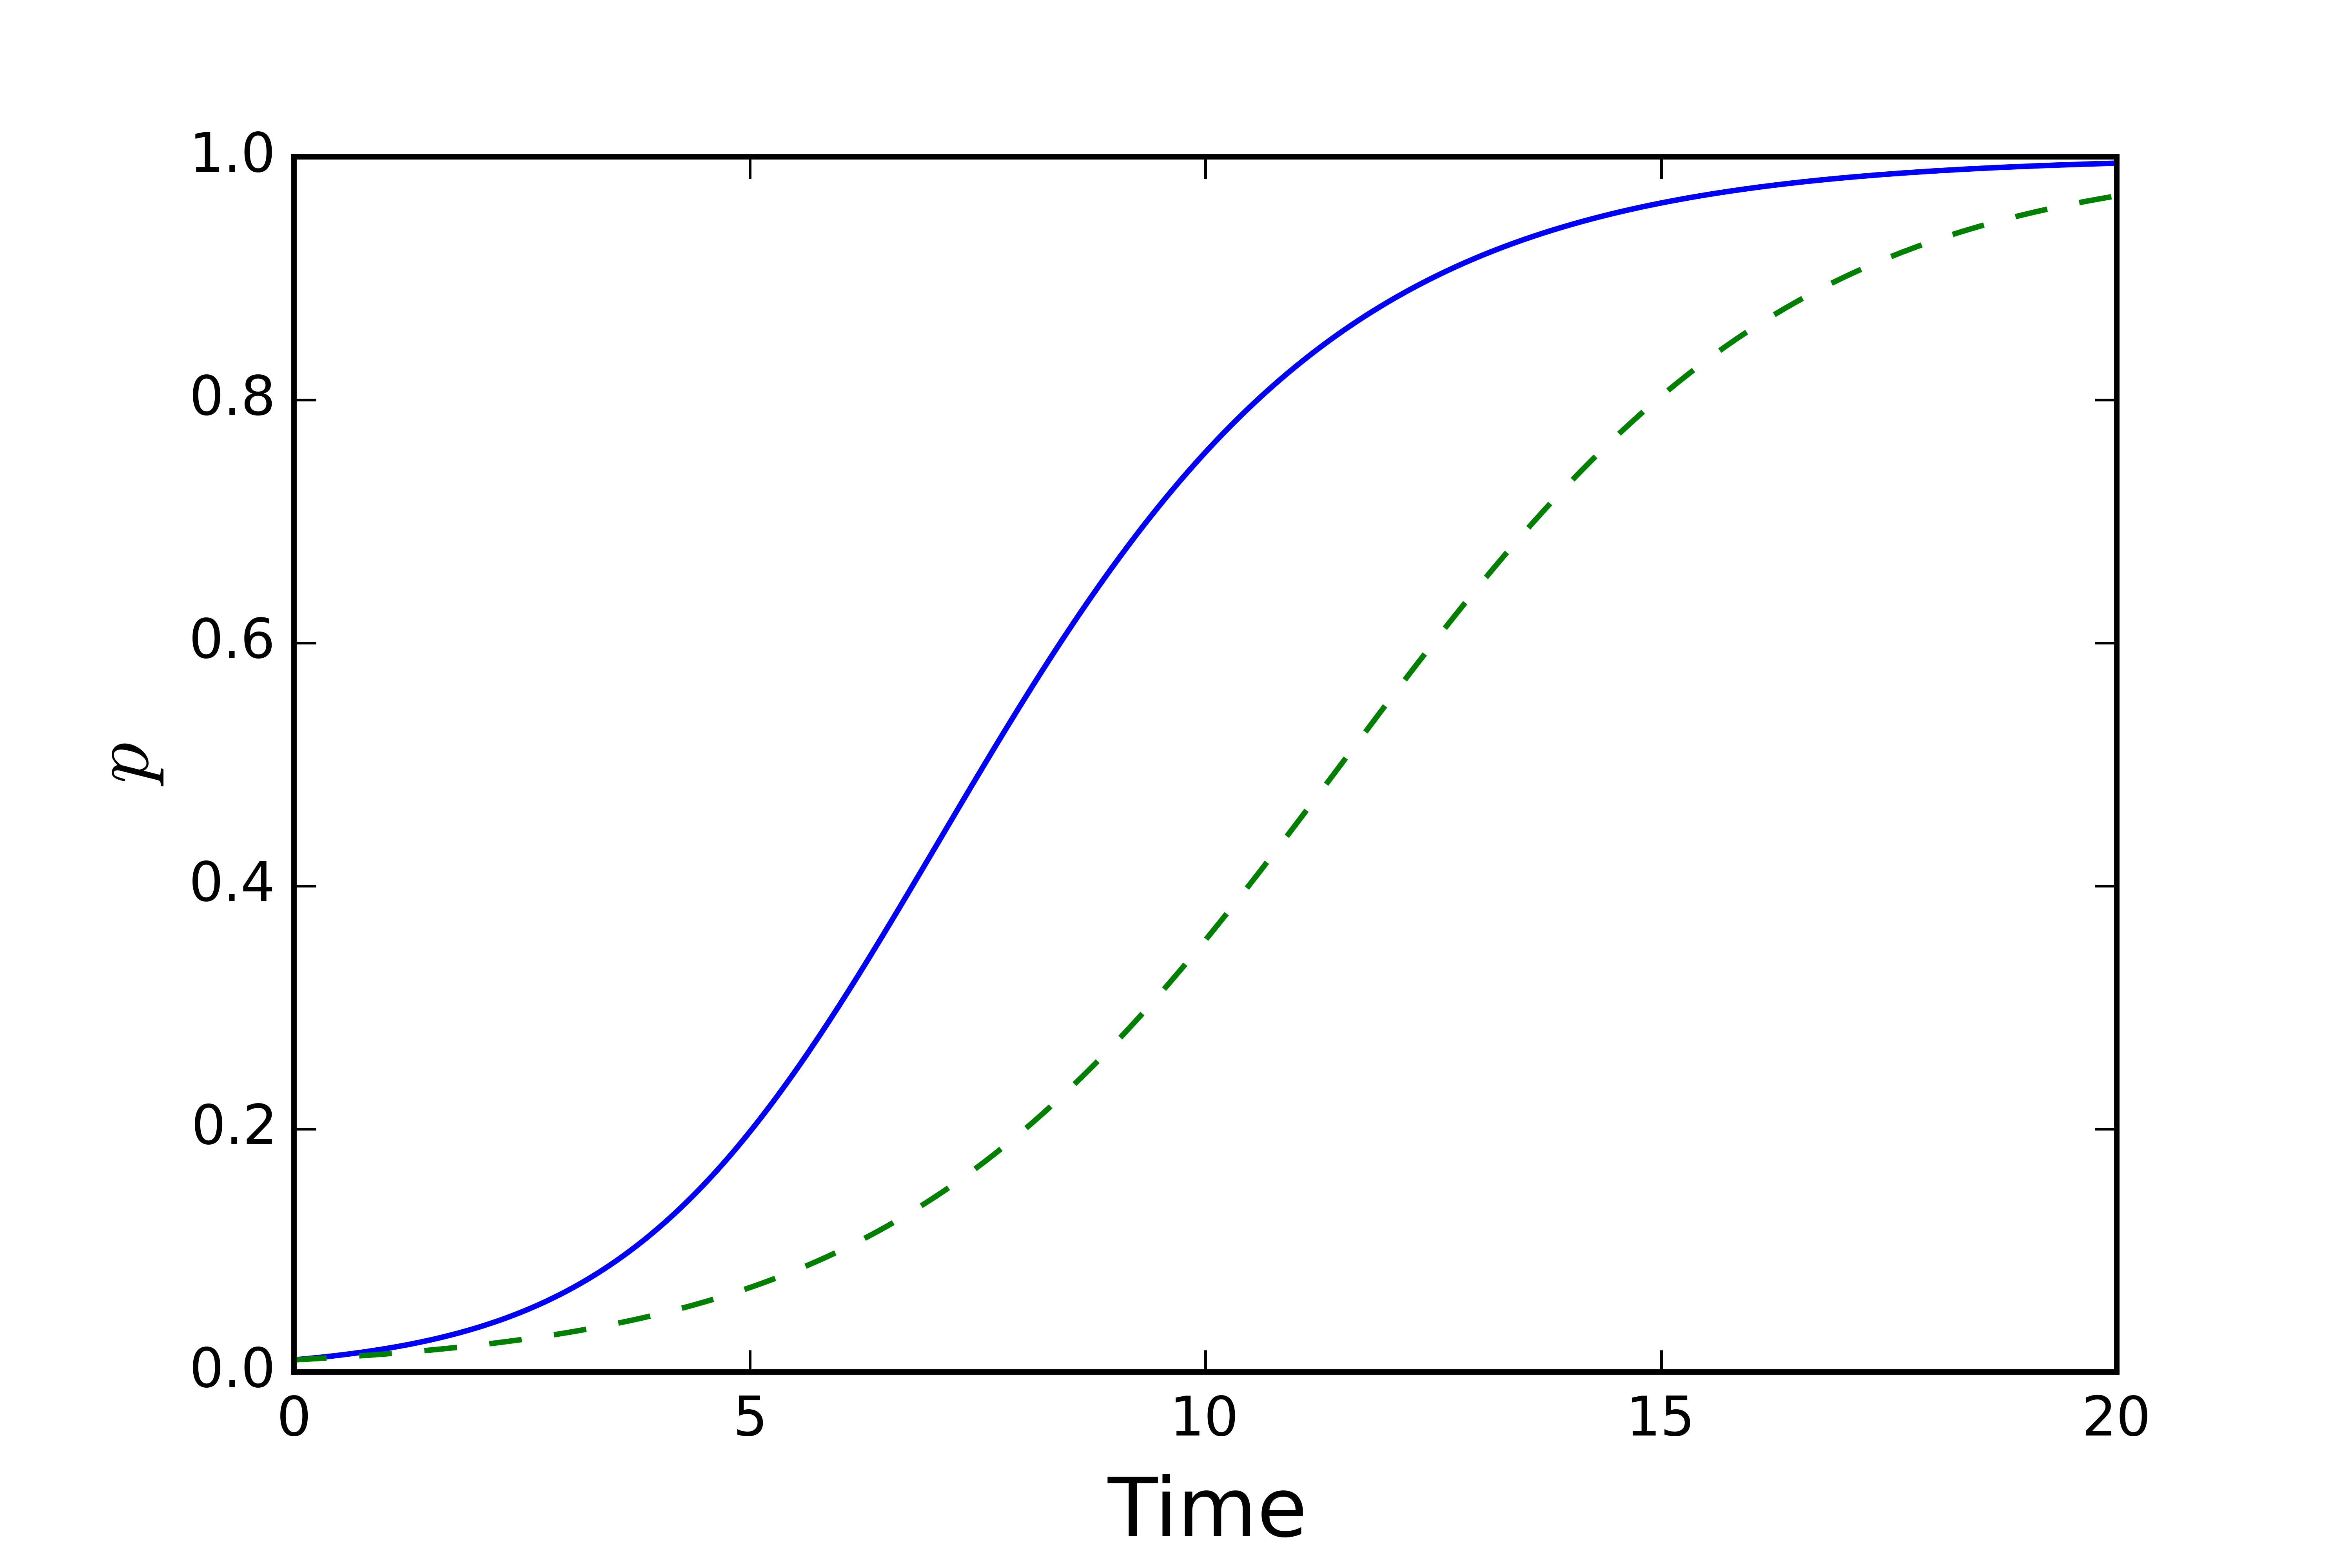
\includegraphics[width=.75\textwidth]{lrp-log.png}\\
\end{center}
	\caption{Solution to acquisition dynamics and logistic model (dashed) from same starting point with $s=.4$}
	\label{lrp-log}
\end{figure}


In many cases the predictions of the two underlying models may not be distinguishable. But, it is certainly possible that we might detect quantitative evidence for the acquisition dynamics. For example for selection coefficients $s \approx 1$ the acquisition dynamics are asymmetric, unlike the logistic, which is perfectly symmetric. This can be seen in the first few solutions in Figure \ref{lrp-gain}. In the context of regression this could potentially lead to quantitative patterns such as heteroscedastic residuals. For example, if we take the acquisition dynamics as a generative model, then fit of the logistic model may systematically under or overestimate the rate of change at different points. We leave investigating this possibility for future research. 

For the second set of rest points, where both grammars have equal independent evidence $s=0$, all distributions over grammars are rest points. All states are \emph{weakly} or \emph{lyupanov stable} in the sense that though the dynamics do not carry the population to a state, the also do not carry the population away from it. Now, we might wonder whether these seemingly knife-edge cases are likely if even possible. However, these cases have a natural interpretation and one that will be particular relevant to the formal cycle. That is, they describe cases where the difference between two grammars hinges on the expression of a single syntactic position. If two grammars correspond to two ways of expressing that position, then the output of each will be incompatible with the other. That is, they will be totally mutually incompatible grammars, rather than only partially incompatible grammars. This can be visualized as in Figure \ref{grammars-incompatible}, which stands in contrast with Figure \ref{grammars-evidence}. In other words, where two grammars vary parametrically at the appropriate level, the dynamics predict a kind of weak stability.

\begin{figure}
\begin{center}
        \begin{tikzpicture}
	  \node (A) [draw,circle,minimum size=4cm]  at (0,0) {$\alpha_1$};
	  \node (G1) [above of=A] {$G_1$};
	  \node [draw,circle,minimum size=4cm] (B) at (0:5cm) {$\alpha_2$};
	  \node (G2) [above of=B] {$G_2$};
	\end{tikzpicture}         
    \end{center}
\caption{Two totally incompatible grammars}
\label{grammars-incompatible}
\end{figure}


So, we determined the acquisition dynamics resulting from the variational model and showed how it exhibits a kind of frequency-independent selection. That is, in most cases only a single grammar is stable. We showed how the resulting dynamics resembles the logistic model of growth. We also noted a crucial exception to this rather robust behavior that leads to a weak kind of stability.  With this in mind, we now turn to an analysis of the syntactic structures underlying the formal cycle.

\section{The syntactic structures of the formal cycle}

There are a range of ways of analyzing the syntactic structures underlying the formal cycle.\footnote{For example, different analyses have suggested varying levels of detail in the number and realization of stages, ranging from three stages  \citep{burridge1983,bernini-ramat1996,haspelmath1997,frisch1997,zanuttini1997,horn:1989,hoeksma1997,horn2001,roberts-roussou2003,vanderAuwera-neuckermans2004,mazzon2004,willis2005,lucas2007,jager2008,wallage2008}, to four stages \citep{dahl:1979,schwegler1988,schwegler1990,schwenter2005,schwenter2006}, up to five stages \citep{honda2000,beukema1999,vanderAuwera-neuckermans2004,zeijlstra2004}.} Here we focus on the analysis presented in \cite{frisch1997}, which treats the formal cycle as the result of two independent morphological changes. First, we present the theoretical details of the analysis. We then note corpus evidence in favor of this treatment.

% Finally, we explicitly state the grammars posited to underly the formal cycle.


\cite{frisch1997} takes Pollock's \citeyearpar{pollock1989} analysis of  negation as a starting point, assuming that negation constitutes its own phrase, with a fully projected structure like that in Figure \ref{negp}: Neg$^0$ is the head of the phrase, Spec is its specifier, and XP is a sister phrase such as a verb phrase.  In particular, Frisch assumes that this underlying structure is always present  \citep{haegeman1995}. The formal cycle simply consists in changes to how the positions in this underlying structure are expressed.\footnote{This is a more localized version of the  \emph{cartographic approach} advocated by \cite{rizzi1997}, which posits a universal syntactic structure. The locus of variation between languages under this conception is how that universal structure is expressed.}


\begin{figure}
        \Tree [.NegP [. Spec ]
        [.Neg$'$ Neg$^0$
        XP ] ]

\caption{The structure of the Negative Phrase} 
\label{negp}
\end{figure}

%However, he treats the embracing form as epiphenomenal, arising from two independent morphological changes in a fixed underlying structure. The assumption of a fixed structure can be stated as in Haegeman's \citeyearpar{haegeman1995} \emph{Neg-criterion} on negative phrases.
%
%\begin{definition}
%The Neg-criterion
%\begin{enumerate}
%	\item Each Neg $X^0$ must be in a spec-head relationship with a Neg operator.
%	\item Each Neg operator must be in a spec-head relationship with a Neg $X^0$.
%	\item Neg-operator: a NEG phrase in a scope position
%	\item Scope position: a left-peripheral A -position (i.e. XP-adjoined or Spec).
%\end{enumerate}
%\end{definition}

%This criterion simply requires that the negative phrase always have the full structure as in Figure \ref{negp}, including a head and a specifier. The strongest form of this assumption posits a universal syntactic structure, where the locus of variation between languages lies in how this universal structure is expressed (cf. the \emph{cartographic} approach advocated by \citealt{rizzi1997}, \emph{inter alia}).

At the first stage of the formal cycle the negative head is expressed as \emph{ne} whereas the specifier is a phonologically null operator $\varnothing$. The syntactic structure according to this morphological analysis can be seen in Figure \ref{stage1morphology}. Sentential structure at stage one of the formal cycle in Old English is illustrated in Figure \ref{sentence1morphology}, where a strikethrough indicates successively upwards head movement. The result is purely pre-verbal negation.

%$_{[+\text{NEG}]}$
\begin{figure}
        \Tree [.NegP [.XP $\varnothing$ ]
        [.Neg$'$ [.Neg \emph{ne}
        ] [.VP \edge[roof]; {...} ] ] ]

\caption{Stage one of the formal cycle according to morphological analysis}
\label{stage1morphology}        
\end{figure}


\begin{figure}
        \Tree [.TP [.DP ic ] [.T$'$ [.V+Neg+T {ne secge} ] [.NegP $\varnothing$
        [.Neg$'$ [.\sout{V+Neg}
        ] [.VP \sout{V} ... ] ] ] ] ]

\caption{Sentential structure at stage one of the formal cycle according to morphological analysis}
\label{sentence1morphology}
\end{figure}

The transition to the second stage in the formal cycle stems from a change in the realization of the specifier of the negative phrase. Namely, the specifier is no longer expressed by a null operator, but instead by \emph{not}, as can be seen in Figure \ref{stage2morphology}. Sentential structure at the second stage of the formal cycle in Middle English is illustrated in Figure \ref{sentence2morphology}, which results in pre- and post-verbal negative elements.


\begin{figure}
        \Tree [.NegP [.XP \emph{not} ]
        [.Neg$'$ [.Neg \emph{ne}
        ] [.VP \edge[roof]; {...} ] ] ]

\caption{Stage two of the formal cycle according to morphological analysis}
\label{stage2morphology}        
\end{figure}


\begin{figure}
        \Tree [.TP [.DP I ] [.T$'$ [.V+Neg+T {ne seye} ] [.NegP \emph{not}
        [.Neg$'$ [.\sout{V+Neg}
        ] [.VP \sout{V} ... ] ] ] ] ]

\caption{Sentential structure at stage two of the formal cycle according to morphological analysis}
\label{sentence2morphology}
\end{figure}

%At this point in the formal cycle we might wonder whether the introduction of two negative elements is problematic. That is, if each element contributes semantic negation in its own right, then the two might cancel each other out. In classical terms, a doubly negated proposition is logically equivalent to the bare proposition.  To circumvent this problem \cite{frisch1997} argues for the \emph{Economy of Projection} principle posited independently by \cite{speas1994}.

%\footnote{Of course, this equivalence ceases to hold in intuitionistic logic, which abandons the elimination of double negation $\neg \neg p \leftrightarrow p$ and the law of the excluded middle $p \vee \neg p$ in favor of a proof-theoretic approach.}

%\begin{definition}
%Economy of Projection principle
%\begin{enumerate}
%	\item Project a phrase XP only if XP has content
%\end{enumerate}
%\end{definition}

%This principle simply states that we can only posit syntactic structure where we have some evidence for it. In this case, the negative phrase is licensed if it contains material in either the head or the specifier. In other words, neither element is necessary for the phrase to occur, so neither can be responsible for the contribution of negative meaning by itself. Rather, it is the negative phrase as a whole that contributes semantic content of negation to the sentence. This can be seen in Figures \ref{stage1morphology} and \ref{stage2morphology} where it is the entire negative phrase that carries the $[+\text{NEG}]$ feature of semantic negation.

The transition from the second stage to the third and final stage of the formal cycle is simply a a matter of whether the negative head is expressed via lexical content or by some null head $\varnothing$. The structure of the negative phrase at the third stage is shown in Figure \ref{stage3morphology}, and sentential structure at this final stage in Late Middle English is shown in Figure \ref{sentence3morphology}. 

%Subsequent stages of negation can be derived by considering the loss of verb raising and the rise of \emph{do}-support.

\begin{figure}
        \Tree [.NegP [.XP \emph{not} ]
        [.Neg$'$ [.Neg $\varnothing$ ]
        [.VP \edge[roof]; {...} ] ] ] 

\caption{Stage three of the formal cycle according to morphological analysis}
\label{stage3morphology}
\end{figure}

\begin{figure}
        \Tree [.TP [.DP I ] [.T$'$ [.V+Neg+T {say} ] [.NegP \emph{not}
        [.Neg$'$ [.\sout{V+Neg}
        ] [.VP \sout{V} ... ] ] ] ] ]

\caption{Sentential structure at stage three of the formal cycle according to morphological analysis}
\label{sentence3morphology}
\end{figure}

Similar morphological approaches to the formal cycle are adopted by \cite{roberts-roussou2003} and \cite{zeijlstra2004}. The shared aspect of these morphological analyses is the assumption that the underlying syntactic structure remains stable, but the realizations of particular positions within that structure changes. Importantly, since this is the only locus of change, the transitions that constitute the cycle are independent of each other. That is, the fact that both \emph{ne} and \emph{not} show up in the embracing \emph{\textcolor{blue}{ne...not}} form is simply the coincidental product of two forms waxing and waning at the same time.

\cite{frisch1997} tests this theoretical prediction using the trajectory of negation in Middle English in the Helsinki corpus of Middle English. He notes that if the two transitions are independent of each other, then the co-occurrence of \emph{ne} and \emph{not} in the negative phrase should be the product of the probabilities of each occurring. 

\begin{equation}
	P(\emph{\textcolor{blue}{ne...not}}) = P(\emph{ne})P(\emph{not})
\end{equation}
That is, the probability of \emph{\textcolor{blue}{ne...not}} is the probability of two independent events \emph{ne} and \emph{not}. This is in fact what Frisch finds.\footnote{Calculating these probabilities requires some adjustment for things like instances of adverbial \emph{not} among others. See \citet[32-47]{frisch1997} for the details.} So the formal cycle can be conceived of as two changes in the expression of positions within an underlying structure. In what follows, we will assume that grammatical knowledge is represented as in Figures \ref{stage1morphology}, \ref{stage2morphology}, and \ref{stage3morphology}. That is, under the assumption of a constant underlying structure, a grammar is characterized by the mapping from the syntactic positions in the negative phrase to lexical items. With these definitions in place, we turn to the actual trajectories of the transitions of the formal cycle in English.


%Frisch estimates the probabilities required to test this prediction in the following manner. First, he estimates the total tokens of \emph{ne} by simply counting the appearances of \emph{ne}. Second, the number of relevant \emph{not} tokens has to be adjusted to exclude adverbial tokens of \emph{not}, which are not part of the negative phrase. Frisch uses the distribution of the adverbial \emph{never} pre- and post-verbally to estimate the proportion of adverbil \emph{not}. Namely, if adverbial \emph{not} is distributed in similar proportions pre- and post-verbally, then the total number of adverbial \emph{not} tokens can be estimated from the total number of pre-verbal tokens. With this adjustment, the probability of both \emph{ne} and \emph{not} can be calculated and compared to their joint probability. Treating the embracing form in this manner yields a good fit to the data.

%\footnote{See \cite[52]{frisch1997} Table 13 for details of the $\chi ^2$ test results. See Tables 9, 10, and 11 for the construction of Table 13.}

%If the appearance of \emph{ne} and \emph{not} together as \emph{\textcolor{blue}{ne...not}} is simply coincidental, then how are we to characterize the grammatical knowledge underlying the different stages of the formal cycle? I


%So, the grammar at the first stage of the formal cycle maps the head of the negative phrase to \emph{ne} and the specifier to a null operator $\varnothing$, the grammar at the second stage of the formal cycle maps the head to \emph{ne} and the specifier to \emph{not}, and the grammar at the third stage of the formal cycle maps the head to a null element $\varnothing$ and the specifier to \emph{not}.

%\begin{equation}
% \mbox{$G_1 : $}
%\left\{
%	\begin{array}{ll}
%		Neg^0 \rightarrow ne\\
%		Spec \rightarrow \varnothing
%	\end{array}
%\right.
%\end{equation}
%
%\begin{equation}
% \mbox{$G_2 : $}
%\left\{
%	\begin{array}{ll}
%		Neg^0 \rightarrow ne\\
%		Spec \rightarrow not
%	\end{array}
%\right.
%\end{equation}
%
%\begin{equation}
% \mbox{$G_3 : $}
%\left\{
%	\begin{array}{ll}
%		Neg^0 \rightarrow \varnothing \\
%		Spec \rightarrow not
%	\end{array}
%\right.
%\end{equation}
%With these definitions in place, we turn to the actual trajectories of the transitions of the formal cycle in English.

%\footnote{\citet[56]{frisch1997} explicitly assumes that the formal cycle is simply a transition from one method of licensing the negative phrase to another, and ``does not necessitate invoking two underlying grammars (\emph{I-languages} in the sense of \cite{chomsky1986}), as the old and new systems do not vary on a particular parameter." This is, perhaps, a strange characterization insofar as the first and last stages do indeed vary parametrically with regard to whether the head and specifier of the negative phrase are expressed by non-null elements.}


%At the heart of this question is the amount of evidence that a given element expresses negation. At the beginning of the change clearly only the preverbal negator does so. The postverbal reinforcer only emphasizes this negation. Eventually though, the evidence weighs in favor of the postverbal negator alone being the expression of negation. \cite{wallage2008} characterizes this transition in morphosyntactic terms as the loss of a [+NEG] feature on the preverbal negator, along with the concomitant introduction of a [+NEG] feature on the postverbal negator. This then allows for the loss of the preverbal negator given that the negative feature can be found elsewhere in the sentence.


%We can formulate the effect of various amounts of evidence in terms of Yang's \citeyearpar{yang2002} variational model. First, let there be two grammars, $G_{ne}$ and $G_{not}$, that represent the location of the abstract feature at \emph{ne} and \emph{not} respectively. We can represent the relation between the two grammars schematically as in Figure \ref{grammars}. In this case, $\alpha$ indicates the proportion of the linguistic environment that is only compatible with $G_{ne}$, and $\beta$ indicates the portion of the linguistic environment that is only compatible with $G_{not}$. The proportion of the two grammars in the population is governed by the following learning rule, where $p_0$ and $p_t$ represent the proportion of $G_{ne}$ in the population after $0$ and $t$ generations, and $q_0$ and $q_t$ represent the proportion of $G_{not}$ after $0$ and $t$ generations.


\section{Modeling the formal cycle}

%Now a problem of parameter interference immediately arises. Under the parametric representation of grammars, grammar selection is based on independent parameters. By contrast, fitness measure and thus the outcome of learning�reward or punish- ment�is defined on whole grammars.

Now that we have stated the grammars underlying the stages of the formal cycle we can turn to modeling the transitions of the formal cycle. First, we note that given the structure of the grammars posited to underly the formal cycle, we can treat each of the transitions separately. Second, we note that given the composition of the grammars we should expected stability under the acquisition dynamics. Finally, we fit the acquisition model for the two transitions of the formal cycle and note that the parameters are indeed not what the acquisitions dynamics predict. However, we note what a successful explanation of the formal cycle would have to do.

The grammars underlying the formal cycle differ only in the expression of two syntactic positions. This has two important implications. First, if the two changes in how these positions are expressed are independent of each other, then we can treat them as such. That is, we can treat the two transitions of the formal cycle as independent events of competition between two grammars for expressing those positions. In what follows we take this approach, treating both the first and second transitions as cases of the acquisition dynamics with two grammars. Second, if the grammars involved in each transition differ only in the expression of one position, then they are totally mutually incompatible $s=0$. This means that the acquisition dynamics predict stability in the case of both transitions, but this is certainly not what we observe. In fact, this alone suffices as a demonstration that acquisition as we have modeled it here cannot account for either of the transitions of the formal cycle.  That is, given the description of the grammars underlying the stages of the formal cycle, acquisition cannot cause the transitions between them. This means that the qualitative criterion for acquisition serving as a cause of the formal cycle is not met.

However, it is useful to note what would have to be the case for acquisition to explain the empirical trajectories of the two transitions. That is, if we fit the acquisition dynamics to data, the fitted parameters tell us what we would need to find in order to take acquisition as the cause of the formal cycle. We fit the acquisition dynamics to the trajectory of the first transition modeled as the competition of two grammars for the specifier of the negative phrase. In this case we take $G_1$ as $G_\varnothing$ and $G_2$ as $G_{not}$ to be grammars that determine how the specifier of the negative phrase is expressed.  We take instances of \emph{\textcolor{red}{ne}} to be compatible with $G_\varnothing$ and instances of \emph{\textcolor{blue}{ne...not}} and  \emph{\textcolor{green}{not}} to be compatible with $G_{not}$. The parameters to fit are the initial state of the second grammar in the population and the selection coefficient  $s$ that captures the ratio of evidence in favor of the second grammar. 

The last thing that needs to be specified is the notion of time. The solution to the acquisition dynamics is in abstract time units, but how these correspond to the actual time in days, months, or years is unspecified. We could fit this relationship as another parameter in the model, but this would be problematic if we were to find different values for the second transition. Instead, we stipulate a ratio between the units of the dynamics and years where one abstract time unit corresponds to five years. We take this to be a rough approximation of the time between when a learner is born an starts contributing to the linguistic environment, but leave it to further research to gain a better estimate the actual value.

The results of fitting the acquisition dynamics can be seen in Figure \ref{lrp-first}.\footnote{See Appendix C for details.} It is important to note, however, that regardless of how well the fitted model approximates the actual trajectory of the first transition, the parameters are not possible. That is, the second grammar cannot have an advantage over the first given that they differ only in the expression of a single syntactic position, yet this is exactly what would be required for acquisition to explain the first transition. This means that the quantitative criterion for acquisition serving as a cause of the formal cycle is not met. However, for another description of the grammars underlying the stages of the formal cycle, this parameter would need to match our theoretical predictions. That is, if the grammars were specified differently, the selection coefficient $\hat{s}$ would still have empirical content. We should be able to look at a corpus and use the grammatical descriptions to see if it is consistent.

\begin{figure}
\begin{center}
 \includegraphics[width=.75\textwidth]{lrp-first.eps}\\
\end{center}
	\caption{Proportion of $G_{not}$ over time for the first transition of the formal cycle, $\hat{s} = 0.10291529$}
	\label{lrp-first}
\end{figure}

We also fit the acquisition dynamics to the trajectory of the second transition modeled as the competition of two grammars for the head of the negative phrase. In this case we treat $G_1$ as $G_{ne}$ and $G_2$ as $G_\varnothing$.  We take instances of \emph{\textcolor{red}{ne}} and \emph{\textcolor{blue}{ne...not}} to be compatible with $G_{ne}$ and instances of \emph{\textcolor{green}{not}} to be compatible with $G_\varnothing$. The results of fitting the acquisition dynamics can be seen in Figure \ref{lrp-second}.\footnote{We only fit the dynamics to data from the point where there are instances of \emph{\textcolor{green}{not}} in all subsequent years, from 1300 CE onwards. Again, see Appendix C for details.} Again, this means that our second criterion for acquisition serving as a cause of the formal cycle is not met. So, neither of the criteria for acquisition serving as a cause of the formal cycle have been met. That is, the acquisition dynamics do not predict either of the transitions, nor do the parameters of the fitted models agree with the corpus evidence predicted by the grammars.

\begin{figure}
\begin{center}
 \includegraphics[width=.75\textwidth]{lrp-second.eps}\\
\end{center}
	\caption{Proportion of $G_\varnothing$ over time for the first transition of the formal cycle, $\hat{s} = 0.34128455$}
	\label{lrp-second}
\end{figure}


It bears emphasis that these criteria are not specific to the acquisition dynamics we specified nor to the grammatical structures posited to underly the stages of the formal cycle. We could just as well adopt another model of acquisition or the grammatical description of the formal cycle (cf. \citealt{niyogi2006}).  But, abandoning the appealing theoretical properties of the variational model and its acquisition dynamics seems a bit hasty. This is especially true given that we need some model to provide any explanation at all. There are, however, a wealth of options when it comes to grammatical descriptions of the formal cycle, as we noted above. 

For example, \cite{wallage2008} makes a compelling corpus-driven argument for the treatment of the formal cycle as two interdependent morphosyntactic changes. In particular, Wallage treats the first transition as the addition of the post-verbal \emph{not} as well as the change in the formal features of pre-verbal \emph{ne} from an interpretable to an uninterpretable feature \citep{chomsky1995}. This more articulated approach would likely face the same problem regarding the first transition, but might offer insight into the second transition. But, it would also offer an interesting alternative insofar as it takes the locus of variation to be the properties and features of functional categories, according to the so-called \emph{Chomsky-Borer conjecture}, \citep{baker2008}.

But, regardless, for acquisition to explain the formal cycle, both of the criteria we described above have to be met. Not only must both of the transitions be predicted, they must also be modeled in an empirically and theoretically consistent manner. To perhaps belabor the point, we can use the parameters of the fitted models of the transitions to predict the proportion of the different forms of the formal cycle in English over time. The result can be seen in Figure \ref{lrp-combined}, and indeed the predicted forms are a close match to the empirical trajectories that we observe. It is tempting to take this as a reasonably good result. But, the parameter values that generate this result are on their face not compatible with the grammatical structures posited to underly the formal cycle. If we want to explain, rather than just describe historical changes we need models that get the picture right while simultaneously being self-consistent. That is, we not only need to be able to fit parameters, but also to make sure those parameters make sense given our theoretical assumptions about the grammatical knowledge that speakers acquire.


\begin{figure}
\begin{center}
 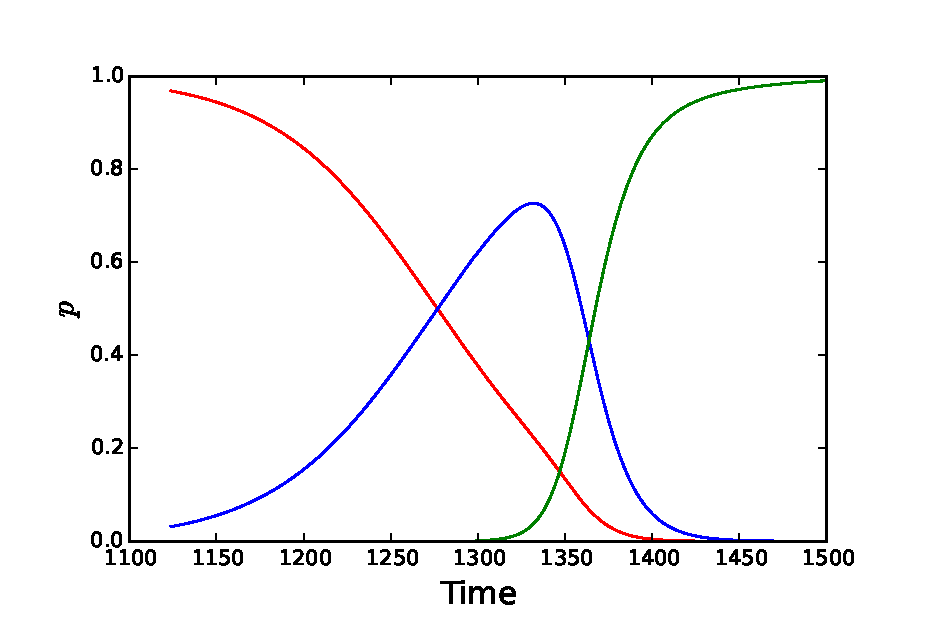
\includegraphics[width=.75\textwidth]{lrp-combined.eps}\\
\end{center}
	\caption{Proportion of \emph{\textcolor{red}{ne}}, \emph{\textcolor{blue}{ne...not}}, and \emph{\textcolor{green}{not}} predicted by the fitted parameters of the acquisition dynamics}
	\label{lrp-combined}
\end{figure}


\section*{Summary}

In this chapter we presented a model of syntactic acquisition, determined its predicted dynamics in a population over time, and fitted it to data from the formal cycle in Middle English. We found that neither the qualitative nor quantitative criteria for taking acquisition as the cause of the formal cycle were met. All together then, it seems that acquisition cannot be taken as a cause of the formal cycle. If this is indeed the case, then it has important consequences for our understanding of the two transitions of the formal cycle.

Regarding the first transition from \emph{\textcolor{red}{ne}} to \emph{\textcolor{blue}{ne...not}}, if acquisition cannot explain it, then use can. That is, given that this transition coincides with the functional cycle, then the explanation of the functional cycle put forward in the previous chapter is the only and necessarily  the best explanation of the observed transition. Alternative analyses of the grammars underlying the formal cycle may change this, they must be both qualitatively and quantitatively accurate and consistent. 

Regarding the second transition from \emph{\textcolor{blue}{ne...not}} to \emph{\textcolor{green}{not}}, neither acquisition nor use can explain it. The transition does not coincide with another functional cycle, \emph{\textcolor{green}{not}} is not restricted to specific contexts.  This leaves us in the strange position of observing a change without an obvious cause.  Absent some mass coincidence, what are we to make of the second transition of the formal cycle? One possibility is that this second transition is not the result of one mass coincidence, but rather the accumulation of many much smaller coincidences.

To see how this might be the case, consider the fact that the acquisition dynamics only predict a weak form of stability in the expected change of the expected behavior of learners in a population. For example, if we relaxed the assumption regarding the size of the population, then the linguistic environment provided to learners would differ slightly from the limit value. For the second transition, suppose that the proportion of $G_\varnothing$ in the actual linguistic environment is slightly higher than expected due to sampling errors. Now, suppose that it is slightly higher in the next generation as well due to sampling errors. If enough of these small coincidences compound over time, one grammar may replace another without ever having more evidence in favor of it. 

Indeed, this possibility has been extensively studied in population genetics in terms of \emph{genetic drift}. That is, when the selection coefficient is zero $s=0$, as is the case in the second transition of the formal cycle, change can come about due to random sampling. Or, in this case, random changes in the probabilities over grammars learned over time. This means that we the second transition might be the result of a series of small coincidences rather than a single improbable one. In the next chapter we turn to means of testing this possibility.
